%!TEX encoding = UTF-8 Unicode

\section{Experimental Results}

\subsection{GLU - Effect Prediction}

Our model permits to make predictions over the effects of actions onto environment objects.

In this experiment, we assume that the Gesture \acp{HMM} provide the discrete value of the recognized action performed by a human agent~(i.e., we enforce a hard decision over the observed action).
%, referring to the possible combination strategies listed in Sec.~\ref{sec:combination}).

\begin{figure}
    \centering
    \subfloat[][Prediction of the movement effect on a small sphere.]
    { 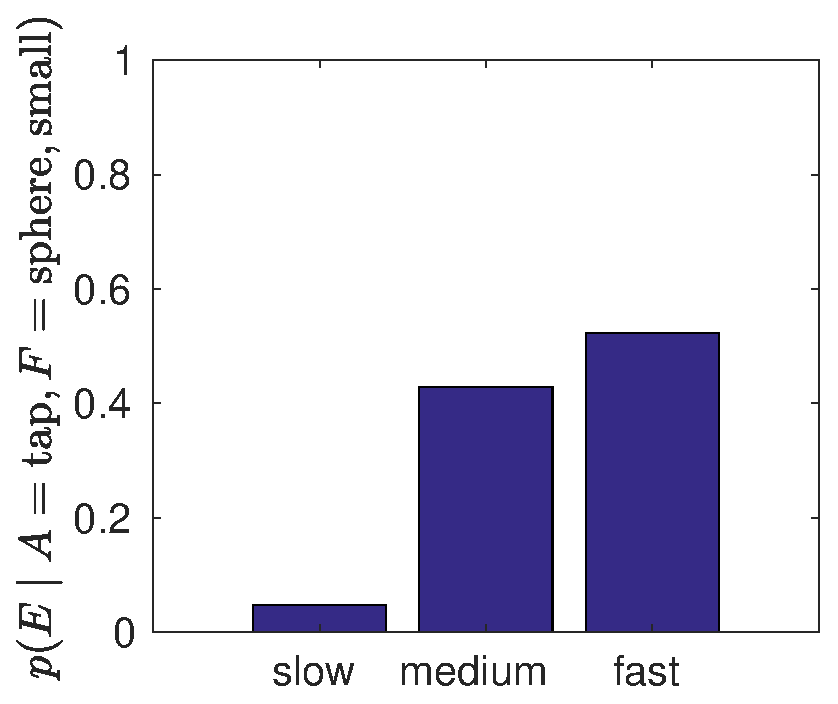
\includegraphics[width=0.45\linewidth]{effectpred_sphere.eps} \label{fig:effect_pred:sphere} } \quad
    %
    \subfloat[][Prediction of the movement effect on a big box.]
    { 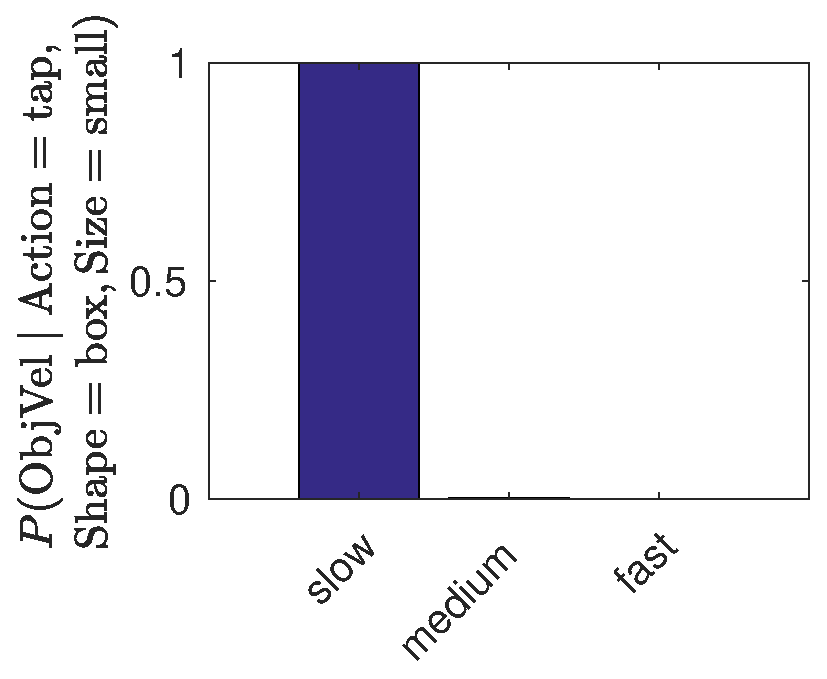
\includegraphics[width=0.45\linewidth]{effectpred_box.eps} \label{fig:effect_pred:box} }
    \caption{Object velocity predictions, given prior information~(from Gesture \acp{HMM}) that the human user performs a tapping action.}
    \label{fig:effect_pred}
\end{figure}


From our combined model of words, affordances and observed actions, we report the inferred posterior value of the Object Velocity effect, given prior information about the action~(provided by the Gesture \acp{HMM}) and also about object features~(Shape and Size). Fig.~\ref{fig:effect_pred} shows the computed predictions in two cases. Fig.~\ref{fig:effect_pred:sphere} shows the anticipated object velocity when the human user performs the tapping action onto a small spherical object, whereas Fig.~\ref{fig:effect_pred:box} displays it when the target object is a big box. Indeed, given the same observed action prior~(lateral tap on the object), the expected movement is very different depending on the physical properties of the target object.

\begin{figure}
\centering
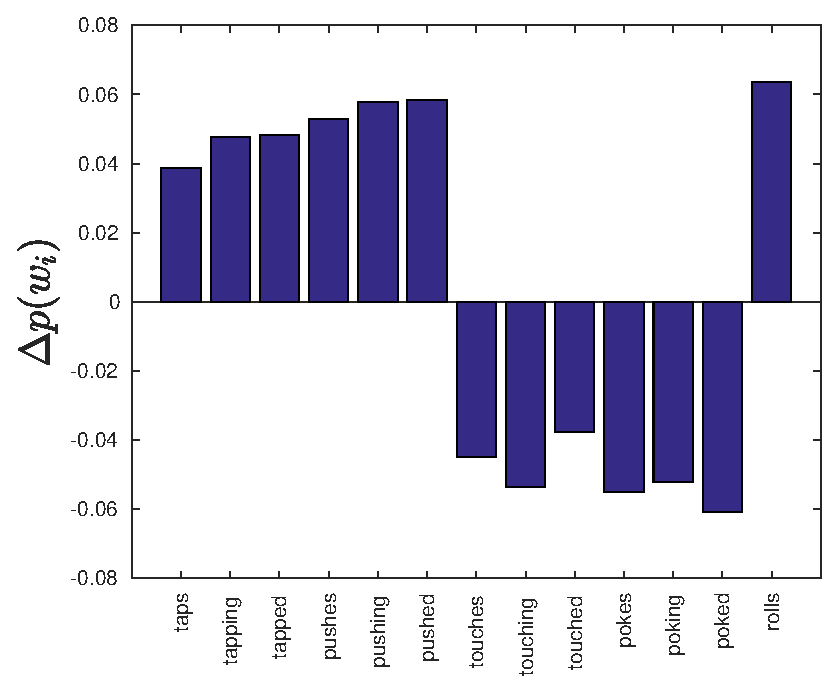
\includegraphics[width=0.9\columnwidth]{partialfig.eps}
\caption{Variation of word occurrence probabilities: $\Delta p(w_i) = p(w_i \mid F, E, A=\text{tap}) - p(w_i \mid F,E)$, where $F = \{\text{Size=big, Shape=sphere}\}$, $E = \{\text{ObjVel=fast}\}$. This variation corresponds to the difference of word probability when we add the tap action evidence~(obtained from the Gesture \acp{HMM}) to the initial evidence about object features and effects. We have omitted words for which no significant variation was observed.}
\label{fig:probdiff}
\end{figure}

\subsection{GLU - Prediction of Words}

Our model permits to make predictions over the associated word descriptions in the presence or absence of an action prior.

As in the previous experiment, we assume that the Gesture \acp{HMM} provide the discrete value of the recognized action performed by a human agent~(i.e., we enforce a hard decision over the observed action).

We compare the associated \emph{verbal description} obtained by the \acl{BN} in the absence of an action prior, with the ones obtained in the presence of one. In particular, we compare the \emph{probability of word occurrence} in the following two situations:
\begin{enumerate}
\item when the robot prior knowledge~(evidence in the \ac{BN}) includes information about object features and effects only: \emph{Size=big, Shape=sphere, ObjVel=fast};

\item when the robot prior knowledge includes, in addition to the above, evidence about the action as observed from the Gestures \acp{HMM}: \emph{Action=tap}.
\end{enumerate}

Fig.~\ref{fig:probdiff} shows the variation in word occurrence probabilities between the two cases, where we have omitted words for which no significant variation was observed in this case. We can interpret the difference in the predictions as follows:
\begin{itemize}
\item as expected, the probabilities of words related to tapping and pushing increase when a tapping action evidence from the Gestures \acp{HMM} is introduced; conversely, the probabilities of other action words~(touching and poking) decreases;

\item interestingly, the probability of the word \emph{rolling}~(which is an effect of an action onto an object) also increases when the tapping action evidence is entered. Even though the initial evidence of case~$1$ already included some effect information~(the velocity of the object), it is only now, when the robot perceives that the physical action was a tap, that the event rolling is associated.
\end{itemize}

\section{Emergence of Verbal Descriptions}

In the previous experiment, we have seen how our model is able to generate word probabilities after having received probabilistic observed evidence.
We now wish to go a step further and generate syntactically correct \emph{sentences}, according to the \ac{CFG} which was employed for recognizing the spoken descriptions in~\cite{salvi:2012:smcb}.

We provide the full specification of the \acf{CFG} in Appendix~\ref{appendix:grammar}.
This grammar is used for TODO COMPLETE\dots
In other words, the grammar is \emph{not} used during the \AffWords{} \ac{BN} learning phase: the speech recognizer used therein assumes a loop of words with no grammatical structure, since the model is based on a bag-of-words assumption, where only the presence or absence of each word in the description is considered.

To examine the generated verbal description, we proceed as follows: we provide evidence to the model~(hard or soft evidence), we extract the generated word probabilities and then we match them to a list of~\SI{1000} possible sentences~(randomly generated according to the \ac{CFG}).
The matching process is described in Appendix~\ref{appendix:grammar}.

For example, if we provide the following evidence the model:
\begin{equation*}
\{\text{Color=yellow, Size=big, Shape=circle, ObjVel=fast}\}
\end{equation*}
we obtain the sentences reported in Table~\ref{tab:generated_sentences_1}.

\begin{table}
    \centering
    \caption{Sentences generated from the evidence $\{\text{Color=yellow, Size=big, Shape=circle, ObjVel=fast}\}$. The higher the score, the better. In the most likely sentence, the correct action-related verb ``taps'' is generated, and the object term ``ball'' is used twice, both in the first part and in the second part of the sentence.}
    \label{tab:generated_sentences_1}
    \begin{tabular}{ll}
    \toprule
    sentence & score \\
    \midrule
    \textbf{baltazar tapped the ball and the ball moves} & \bm{$-0.63813$} \\
    baltazar taps the ball and the sphere is moving & $-0.64636$ \\
    the robot touched the big sphere and the ball is rolling & $-0.64822$ \\
    he taps the sphere and the sphere moves & $-0.65437$ \\
    the robot has poked the ball and the sphere moves & $-0.67455$ \\
    baltazar just tapped the sphere and the sphere is rolling & $-0.71942$ \\
    baltazar taps the sphere and the big ball rolls & $-0.72702$ \\
    baltazar taps the sphere and the yellow sphere rolls & $-0.73154$ \\
    the robot just touched the sphere and the ball moves & $-0.79609$ \\
    baltazar has poked the ball and the ball rolls & $-0.81551$ \\
    \bottomrule
    \end{tabular}
\end{table}
